\documentclass{standalone}
\usepackage{tikz}
\usetikzlibrary{patterns, positioning}


\begin{document}
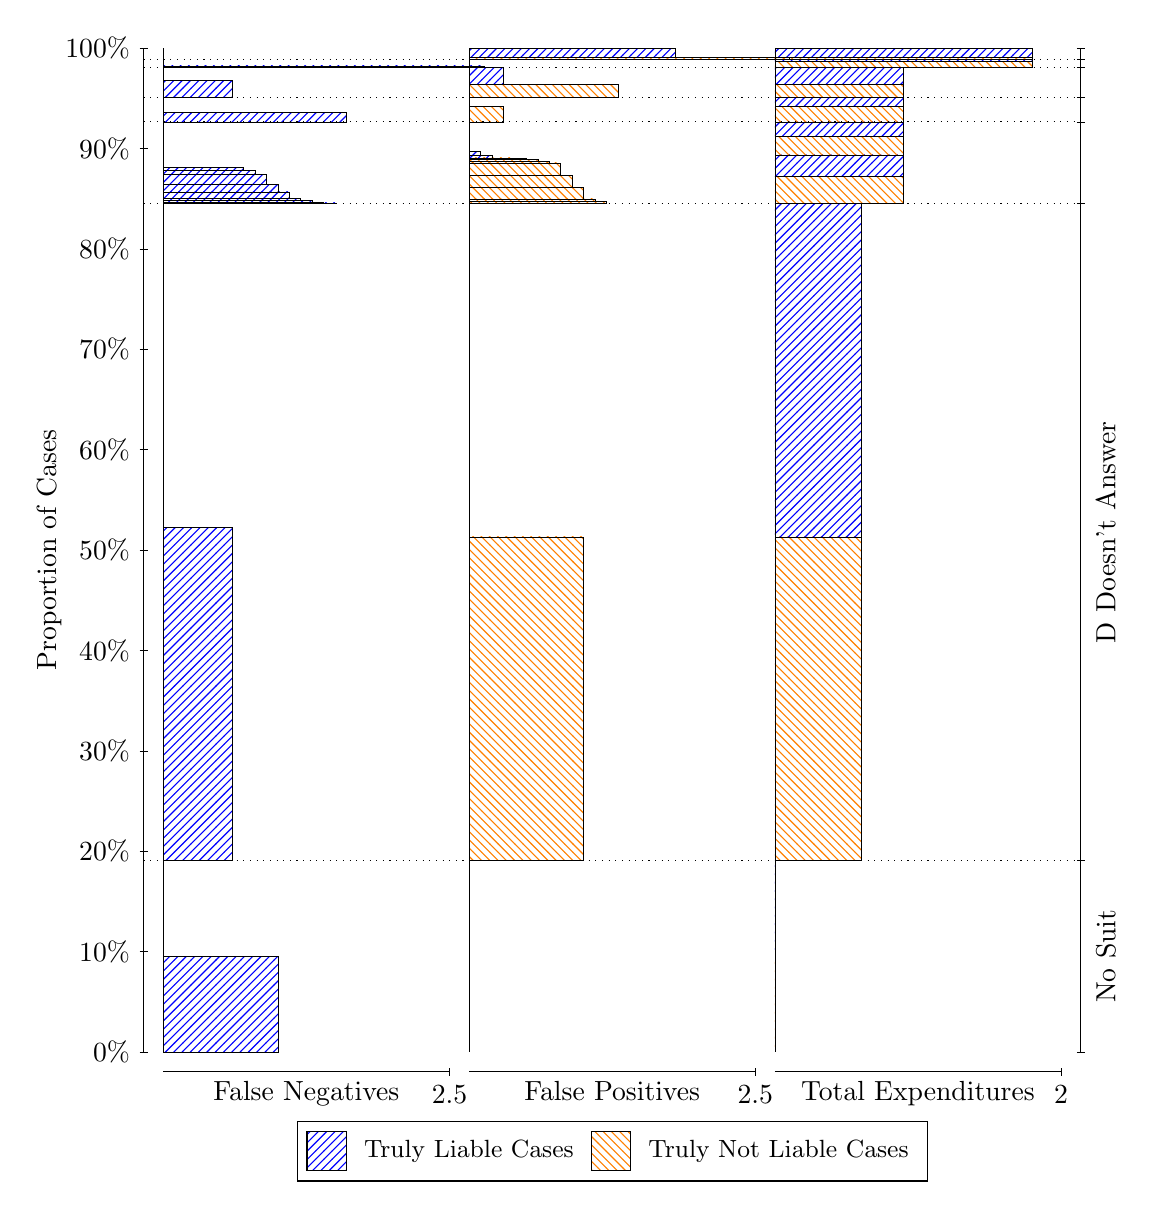
\begin{tikzpicture}
\draw[black, very thin] (1.5,1.75) -- (1.5,14.5);
\node[rotate=90, text=black, anchor=center] at (0.3, 8.125) {Proportion of Cases};
\draw[black, very thin] (1.45,1.75) -- (1.55,1.75);
\node[text=black, anchor=east] at (1.45, 1.75) {0\%};
\draw[black, very thin] (1.45,3.025) -- (1.55,3.025);
\node[text=black, anchor=east] at (1.45, 3.025) {10\%};
\draw[black, very thin] (1.45,4.3) -- (1.55,4.3);
\node[text=black, anchor=east] at (1.45, 4.3) {20\%};
\draw[black, very thin] (1.45,5.575) -- (1.55,5.575);
\node[text=black, anchor=east] at (1.45, 5.575) {30\%};
\draw[black, very thin] (1.45,6.85) -- (1.55,6.85);
\node[text=black, anchor=east] at (1.45, 6.85) {40\%};
\draw[black, very thin] (1.45,8.125) -- (1.55,8.125);
\node[text=black, anchor=east] at (1.45, 8.125) {50\%};
\draw[black, very thin] (1.45,9.4) -- (1.55,9.4);
\node[text=black, anchor=east] at (1.45, 9.4) {60\%};
\draw[black, very thin] (1.45,10.675) -- (1.55,10.675);
\node[text=black, anchor=east] at (1.45, 10.675) {70\%};
\draw[black, very thin] (1.45,11.95) -- (1.55,11.95);
\node[text=black, anchor=east] at (1.45, 11.95) {80\%};
\draw[black, very thin] (1.45,13.225) -- (1.55,13.225);
\node[text=black, anchor=east] at (1.45, 13.225) {90\%};
\draw[black, very thin] (1.45,14.5) -- (1.55,14.5);
\node[text=black, anchor=east] at (1.45, 14.5) {100\%};

\draw[black, very thin] (13.4,1.75) -- (13.4,14.5);
\draw[black, very thin] (13.35,1.75) -- (13.45,1.75);
\node[anchor=west] at (13.35, 1.75) {};
\draw[black, very thin] (13.35,4.1816) -- (13.45,4.1816);
\node[anchor=west] at (13.35, 4.1816) {};
\draw[black, very thin] (13.35,12.523) -- (13.45,12.523);
\node[anchor=west] at (13.35, 12.523) {};
\draw[black, very thin] (13.35,13.563) -- (13.45,13.563);
\node[anchor=west] at (13.35, 13.563) {};
\draw[black, very thin] (13.35,13.875) -- (13.45,13.875);
\node[anchor=west] at (13.35, 13.875) {};
\draw[black, very thin] (13.35,14.251) -- (13.45,14.251);
\node[anchor=west] at (13.35, 14.251) {};
\draw[black, very thin] (13.35,14.359) -- (13.45,14.359);
\node[anchor=west] at (13.35, 14.359) {};
\draw[black, very thin] (13.35,14.5) -- (13.45,14.5);
\node[anchor=west] at (13.35, 14.5) {};

\draw[black, very thin, pattern color=blue, pattern=north east lines] (1.75,1.75) rectangle (3.2033,2.9658);
\draw[black, very thin, pattern color=orange, pattern=north west lines] (1.75,2.9658) rectangle (1.75,4.1816);
\draw[black, very thin, pattern color=blue, pattern=north east lines] (1.75,4.1816) rectangle (2.622,8.4144);
\draw[black, very thin, pattern color=orange, pattern=north west lines] (1.75,8.4144) rectangle (1.75,12.523);
\draw[black, very thin, pattern color=blue, pattern=north east lines] (1.75,12.523) rectangle (3.93,12.532);
\draw[black, very thin, pattern color=blue, pattern=north east lines] (1.75,12.532) rectangle (3.7847,12.542);
\draw[black, very thin, pattern color=blue, pattern=north east lines] (1.75,12.542) rectangle (3.6393,12.562);
\draw[black, very thin, pattern color=blue, pattern=north east lines] (1.75,12.562) rectangle (3.494,12.586);
\draw[black, very thin, pattern color=blue, pattern=north east lines] (1.75,12.586) rectangle (3.3487,12.673);
\draw[black, very thin, pattern color=blue, pattern=north east lines] (1.75,12.673) rectangle (3.2033,12.766);
\draw[black, very thin, pattern color=blue, pattern=north east lines] (1.75,12.766) rectangle (3.058,12.898);
\draw[black, very thin, pattern color=blue, pattern=north east lines] (1.75,12.898) rectangle (2.9127,12.945);
\draw[black, very thin, pattern color=blue, pattern=north east lines] (1.75,12.945) rectangle (2.7673,12.98);
\draw[black, very thin, pattern color=orange, pattern=north west lines] (1.75,12.98) rectangle (1.75,13.563);
\draw[black, very thin, pattern color=blue, pattern=north east lines] (1.75,13.563) rectangle (4.0753,13.682);
\draw[black, very thin, pattern color=orange, pattern=north west lines] (1.75,13.682) rectangle (1.75,13.875);
\draw[black, very thin, pattern color=blue, pattern=north east lines] (1.75,13.875) rectangle (2.622,14.085);
\draw[black, very thin, pattern color=orange, pattern=north west lines] (1.75,14.085) rectangle (1.75,14.251);
\draw[black, very thin, pattern color=blue, pattern=north east lines] (1.75,14.251) rectangle (5.8193,14.274);
\draw[black, very thin, pattern color=orange, pattern=north west lines] (1.75,14.274) rectangle (1.75,14.359);
\draw[black, very thin, pattern color=orange, pattern=north west lines] (1.75,14.359) rectangle (1.75,14.383);
\draw[black, very thin, pattern color=blue, pattern=north east lines] (1.75,14.383) rectangle (1.75,14.5);
\draw[black, very thin, pattern color=orange, pattern=north west lines] (5.6333,1.75) rectangle (5.6333,2.9658);
\draw[black, very thin, pattern color=blue, pattern=north east lines] (5.6333,2.9658) rectangle (5.6333,4.1816);
\draw[black, very thin, pattern color=orange, pattern=north west lines] (5.6333,4.1816) rectangle (7.0867,8.2903);
\draw[black, very thin, pattern color=blue, pattern=north east lines] (5.6333,8.2903) rectangle (5.6333,12.523);
\draw[black, very thin, pattern color=orange, pattern=north west lines] (5.6333,12.523) rectangle (7.3773,12.553);
\draw[black, very thin, pattern color=orange, pattern=north west lines] (5.6333,12.553) rectangle (7.232,12.583);
\draw[black, very thin, pattern color=orange, pattern=north west lines] (5.6333,12.583) rectangle (7.0867,12.728);
\draw[black, very thin, pattern color=orange, pattern=north west lines] (5.6333,12.728) rectangle (6.9413,12.879);
\draw[black, very thin, pattern color=orange, pattern=north west lines] (5.6333,12.879) rectangle (6.796,13.04);
\draw[black, very thin, pattern color=orange, pattern=north west lines] (5.6333,13.04) rectangle (6.6507,13.065);
\draw[black, very thin, pattern color=orange, pattern=north west lines] (5.6333,13.065) rectangle (6.5053,13.087);
\draw[black, very thin, pattern color=orange, pattern=north west lines] (5.6333,13.087) rectangle (6.36,13.097);
\draw[black, very thin, pattern color=orange, pattern=north west lines] (5.6333,13.097) rectangle (6.2147,13.106);
\draw[black, very thin, pattern color=blue, pattern=north east lines] (5.6333,13.106) rectangle (5.924,13.141);
\draw[black, very thin, pattern color=blue, pattern=north east lines] (5.6333,13.141) rectangle (5.7787,13.188);
\draw[black, very thin, pattern color=blue, pattern=north east lines] (5.6333,13.188) rectangle (5.6333,13.563);
\draw[black, very thin, pattern color=orange, pattern=north west lines] (5.6333,13.563) rectangle (6.0693,13.756);
\draw[black, very thin, pattern color=blue, pattern=north east lines] (5.6333,13.756) rectangle (5.6333,13.875);
\draw[black, very thin, pattern color=orange, pattern=north west lines] (5.6333,13.875) rectangle (7.5227,14.041);
\draw[black, very thin, pattern color=blue, pattern=north east lines] (5.6333,14.041) rectangle (6.0693,14.251);
\draw[black, very thin, pattern color=orange, pattern=north west lines] (5.6333,14.251) rectangle (5.6333,14.335);
\draw[black, very thin, pattern color=blue, pattern=north east lines] (5.6333,14.335) rectangle (5.6333,14.359);
\draw[black, very thin, pattern color=orange, pattern=north west lines] (5.6333,14.359) rectangle (9.7027,14.383);
\draw[black, very thin, pattern color=blue, pattern=north east lines] (5.6333,14.383) rectangle (8.2493,14.5);
\draw[black, very thin, pattern color=orange, pattern=north west lines] (9.5167,1.75) rectangle (9.5167,2.9658);
\draw[black, very thin, pattern color=blue, pattern=north east lines] (9.5167,2.9658) rectangle (9.5167,4.1816);
\draw[black, very thin, pattern color=orange, pattern=north west lines] (9.5167,4.1816) rectangle (10.607,8.2903);
\draw[black, very thin, pattern color=blue, pattern=north east lines] (9.5167,8.2903) rectangle (10.607,12.523);
\draw[black, very thin, pattern color=orange, pattern=north west lines] (9.5167,12.523) rectangle (11.152,12.868);
\draw[black, very thin, pattern color=blue, pattern=north east lines] (9.5167,12.868) rectangle (11.152,13.142);
\draw[black, very thin, pattern color=orange, pattern=north west lines] (9.5167,13.142) rectangle (11.152,13.379);
\draw[black, very thin, pattern color=blue, pattern=north east lines] (9.5167,13.379) rectangle (11.152,13.563);
\draw[black, very thin, pattern color=orange, pattern=north west lines] (9.5167,13.563) rectangle (11.152,13.756);
\draw[black, very thin, pattern color=blue, pattern=north east lines] (9.5167,13.756) rectangle (11.152,13.875);
\draw[black, very thin, pattern color=orange, pattern=north west lines] (9.5167,13.875) rectangle (11.152,14.041);
\draw[black, very thin, pattern color=blue, pattern=north east lines] (9.5167,14.041) rectangle (11.152,14.251);
\draw[black, very thin, pattern color=orange, pattern=north west lines] (9.5167,14.251) rectangle (12.787,14.335);
\draw[black, very thin, pattern color=blue, pattern=north east lines] (9.5167,14.335) rectangle (12.787,14.359);
\draw[black, very thin, pattern color=orange, pattern=north west lines] (9.5167,14.359) rectangle (12.787,14.383);
\draw[black, very thin, pattern color=blue, pattern=north east lines] (9.5167,14.383) rectangle (12.787,14.5);
\draw[black, dotted] (1.5,4.1816) -- (13.4,4.1816);
\draw[black, dotted] (1.5,12.523) -- (13.4,12.523);
\draw[black, dotted] (1.5,13.563) -- (13.4,13.563);
\draw[black, dotted] (1.5,13.875) -- (13.4,13.875);
\draw[black, dotted] (1.5,14.251) -- (13.4,14.251);
\draw[black, dotted] (1.5,14.359) -- (13.4,14.359);
\draw[black, very thin] (1.75,1.5) -- (5.3833,1.5);
\node[text=black, anchor=north] at (3.5667, 1.5) {False Negatives};
\draw[black, very thin] (5.3833,1.45) -- (5.3833,1.55);
\node[text=black, anchor=north] at (5.3833, 1.45) {2.5};

\draw[black, very thin] (5.6333,1.5) -- (9.2667,1.5);
\node[text=black, anchor=north] at (7.45, 1.5) {False Positives};
\draw[black, very thin] (9.2667,1.45) -- (9.2667,1.55);
\node[text=black, anchor=north] at (9.2667, 1.45) {2.5};

\draw[black, very thin] (9.5167,1.5) -- (13.15,1.5);
\node[text=black, anchor=north] at (11.333, 1.5) {Total Expenditures};
\draw[black, very thin] (13.15,1.45) -- (13.15,1.55);
\node[text=black, anchor=north] at (13.15, 1.45) {2};

\node[text=black, centered, rotate=90] at (13.72, 2.9658) {No Suit};
\node[text=black, centered, rotate=90] at (13.72, 8.3523) {D Doesn't Answer};






\draw (7.449999999999999,1.5) node[draw=none] (baseCoordinate) {};
\begin{scope}[align=center]
        \matrix[scale=0.5, draw=black, below=0.5cm of baseCoordinate, nodes={draw}, column sep=0.1cm]{
            \node[rectangle, draw, minimum width=0.5cm, minimum height=0.5cm, pattern color=blue, pattern=north east lines] {}; &
            \node[draw=none, font=\small, text=black] (B) {Truly Liable Cases}; &
            \node[rectangle, draw, minimum width=0.5cm, minimum height=0.5cm, pattern color=orange, pattern=north west lines] {}; &
            \node[draw=none, font=\small, text=black] (B) {Truly Not Liable Cases}; \\
            };
\end{scope}

\end{tikzpicture}
\end{document}